
\section{Mobile application for data gathering and model testing}

The application was written for Android devices supporting Android 8.1 or newer. As of 2024 \cite{androidStats}, more than 93\% of Android devices should be compatible. The Android platform was chosen, as it was easier to test on and find a study group of the Android users as opposed to the iOS users (according to \cite{operatingSystemDistribution} , significantly more people in Poland, where the researchers are based in, use Android devices).

Technology used in the mobile application itself was Jetpack Compose, which is quoted by Google to be "Android’s recommended modern toolkit for building native UI" \cite{jetpackCompose}. Language used was Kotlin. Persisence was achieved by using Android Room, which provided an abstraction layer over SQLite database, which was used for data collection.

TODO for KM: add statistics sources (Internet), some technicals about the inner workings of the app. How the data is stored, what is gathered and when. If you have any doubts, feel free to ask about any methods/composables. I will be updating method descriptions/docs soon -- JG

\subsection{Model View ViewModel and DataStore}

The application uses Model-View-ViewModel (MVVM) provided by Jetpack Compose design pattern to support a clear separation of concerns. 
\begin{itemize}
	\item \textbf{Model:} Data is modeled using \texttt{KeyPressEntity} class, which represents a single key press event. It includes: 
	\begin{itemize}
		\item \textbf{Key} (\texttt{String}): The key pressed by the user.
		\item \textbf{Press Time} (\texttt{Long}): The exact timestamp of the key press event.
		\item \textbf{Duration} (\texttt{Long}): The time elapsed since the last key press event.
		\item \textbf{Accelerometer Data} (\texttt{Float}): Currently unused but useful for future developing of the project. 
	\end{itemize}
	\begin{figure}[h!]
		\centering
		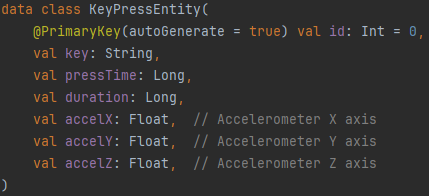
\includegraphics[width=0.8\linewidth]{images/DataModel.png}
		\caption{KeyPressEntity.kt}
		\label{fig:data_model_view}
	\end{figure}
	
	The \texttt{KeyPressEntity} is stored in a local SQLite database via Room.
	
	\item \textbf{View:} The user interface is implemented using \textbf{Jetpack Compose}, a declarative UI framework. Key components of the view contain:
	\begin{itemize}
		\item \textbf{Input Fields:} Lets users enter their credentials (University ID) and use the application for training or testing by pressing keys. 
		\item \textbf{Completion progress:} Informs users on what phase they are and displays progress of completion, linked to the \texttt{phasesCompleted} state in the \texttt{MainViewModel}.
		\item \textbf{Buttons:} Used for logging in, logging out, jumping phases and sending or downloading the data collected through training or testing stage.
	\end{itemize}
	\item \textbf{ViewModel:} This role is fulfilled by \texttt{MainViewModel}, which manages the application logic, handles interactions between the model and the view, and maintains the state of the app. \newline
	The \texttt{MainViewModel} class manages this operations through:
	\begin{itemize}
		\item \textbf{Logic Handling:} Methods such as \texttt{login()}, \texttt{logout()}, \texttt{clearDatabase()}, and \texttt{onKeyPress()} are responsible for managing user state and data.
		\item \textbf{State Management:} Stores states \texttt{isLoggedIn}, \texttt{username}, and \texttt{phasesCompleted}, which are used to dynamically update the user interface.
		\item \textbf{Data Management:} Connects with the \texttt{keyPressDao} database to process data. \texttt{onKeyPress} saves key press events into the database, \texttt{exportDataToTsv} exports the collected data into TSV files.
	\end{itemize}
\end{itemize}
In the app \textbf{DataStore} is used for storing login state and the user's ID. It has been implemented in \texttt{UserPreferences} class, and stores data such as:
\begin{itemize}
	\item \texttt{LOGGED\_IN\_KEY} - login state
	\item \texttt{USERNAME\_KEY} - user's ID.
\end{itemize}
\begin{figure}[h!]
	\centering
	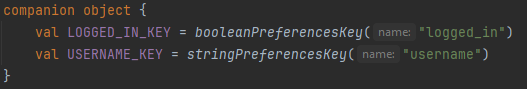
\includegraphics[width=0.8\linewidth]{images/CompanionObject.png}
	\caption{UserPreferences.kt}
	\label{fig:companion_object_view}
\end{figure}
This data is stored in the app's preferences file and can be accessed via dataStore object using:

\begin{itemize}
	\item \texttt{isLoggedIn} - returns login state as \texttt{Flow<Boolean>}
	\item \texttt{username} - returns user's ID as \texttt{Flow<String>}
	\item \texttt{setLoggedIn()} - saves login state and user's ID into DataStore
\end{itemize}

\begin{figure}[H]
	\centering
	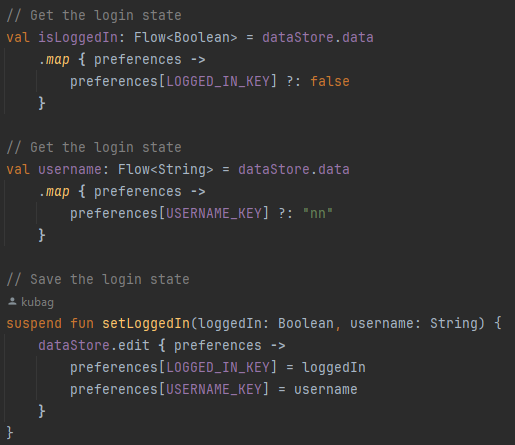
\includegraphics[width=0.8\linewidth]{images/UPFunctions.png}
	\caption{UserPreferences.kt}
	\label{fig:user_preferences_functions_view}
\end{figure}

The use of DataStore enabled the data to be stored securely, accessed and modified easily, and it is always available, which makes it a reliable and efficient way to manage user preferences and app state.

\subsection{User Interface Design}
The application design follows a minimalistic approach to make it intuitive and easy to use for everyone. 
\begin{itemize}
	\item \texttt{Login Screen} \ref{fig:login_screen} \newline
	After launching the application for the first time, the user is presented with the \texttt{Login screen}. It contains \texttt{TextInput} field for entering the university ID, which was evenly distributed among contributors to simplify testing, and the \texttt{Log in} button which stores the ID and navigates the user to the \texttt{Home Screen}.
	\item \texttt{Home Screen} \ref{fig:home_screen} \newline
	\item \texttt{Training Screen} \ref{fig:training_screen} \newline
	\item \texttt{Testing Screen} \ref{fig:testing_screen} \newline
\end{itemize}


\begin{figure}[H]
	\centering
	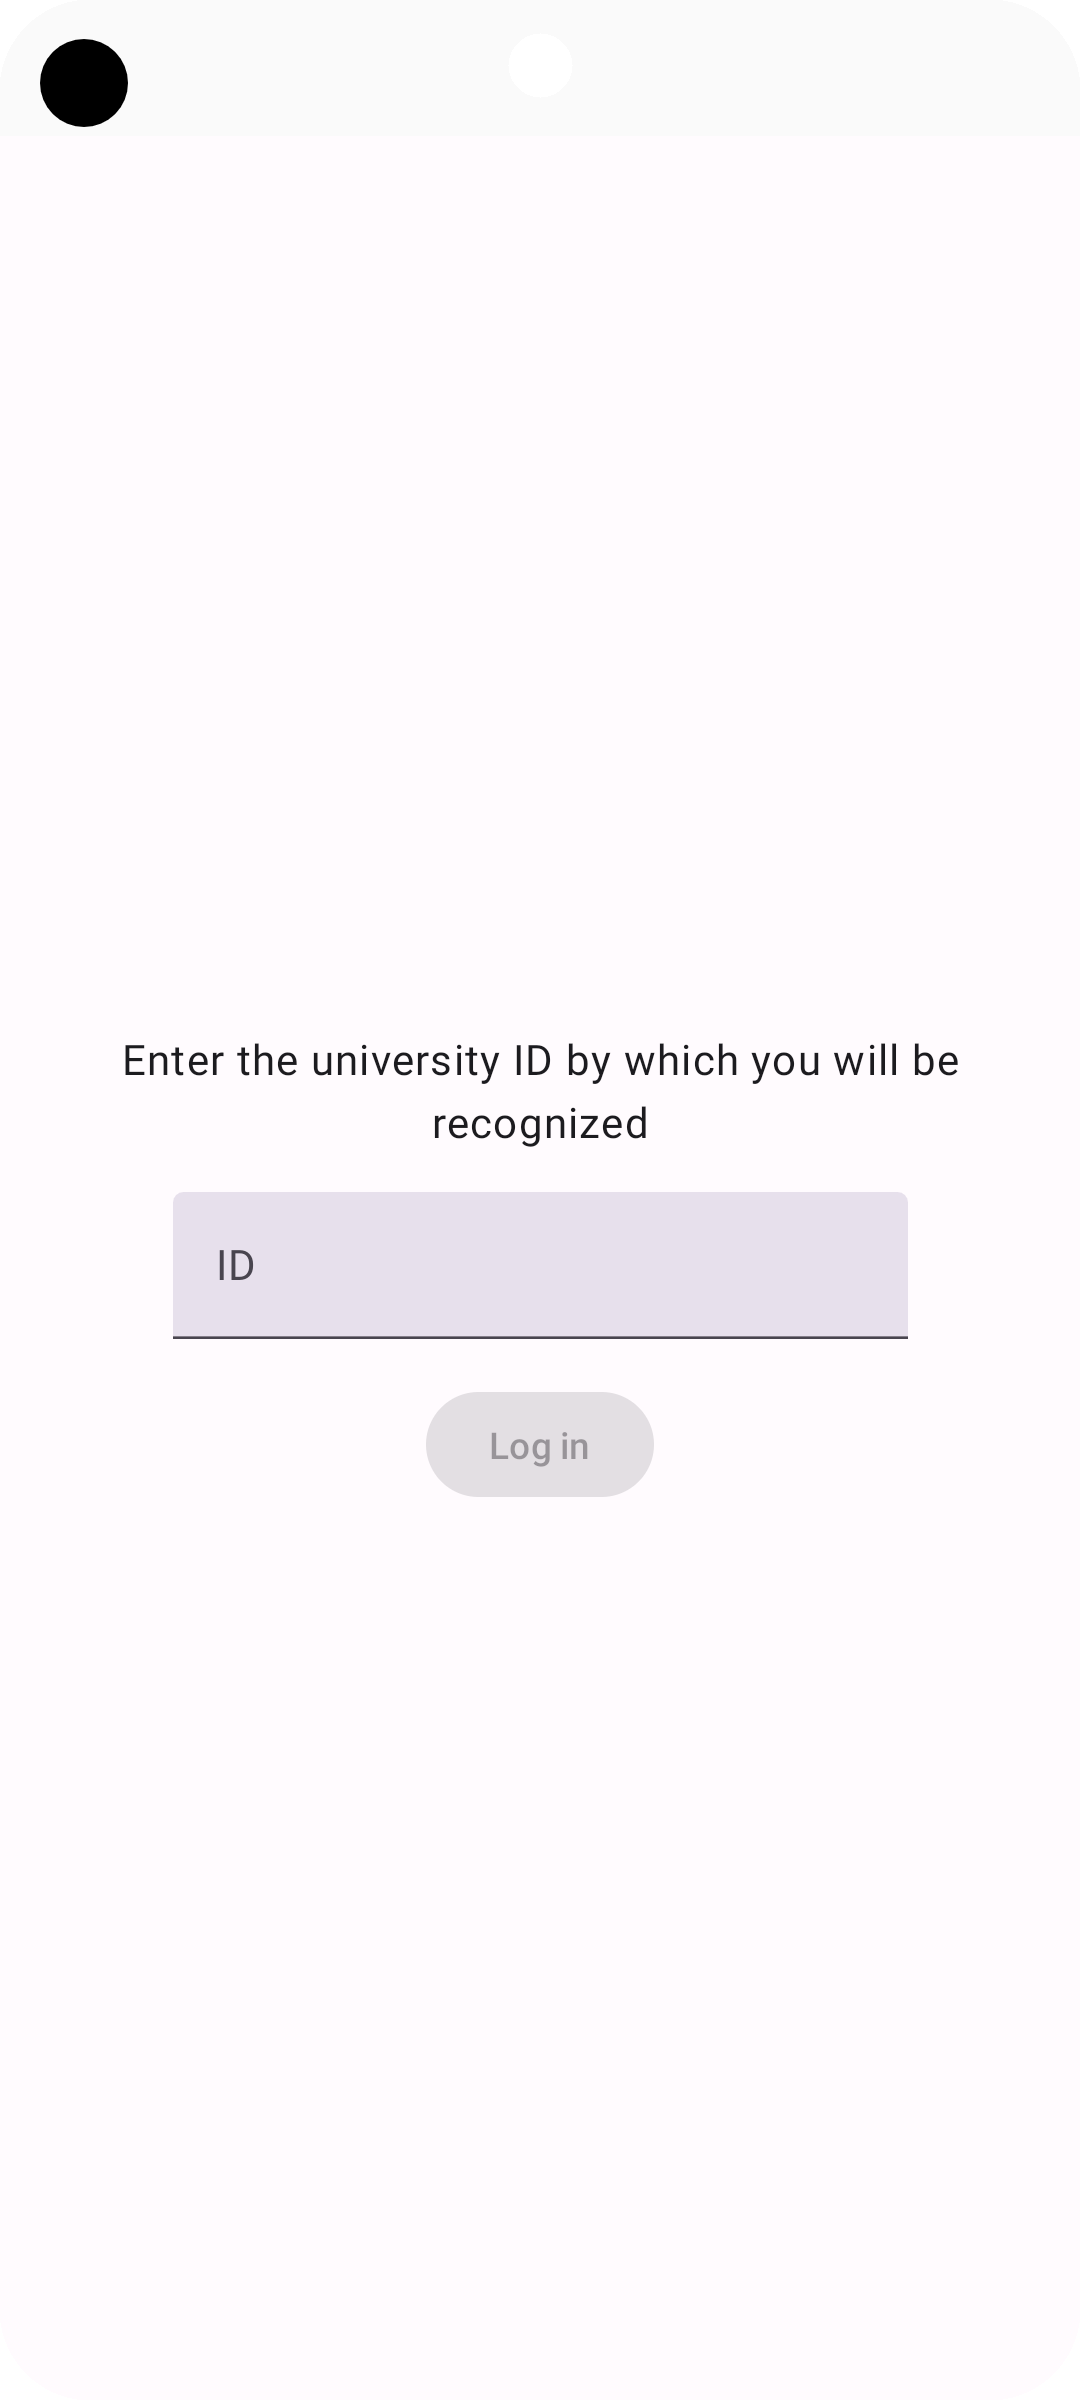
\includegraphics[width=0.32\linewidth]{images/login_screen.png}
	\caption{Login screen}
	\label{fig:login_screen}
\end{figure}

\begin{figure}[H]
	\centering
	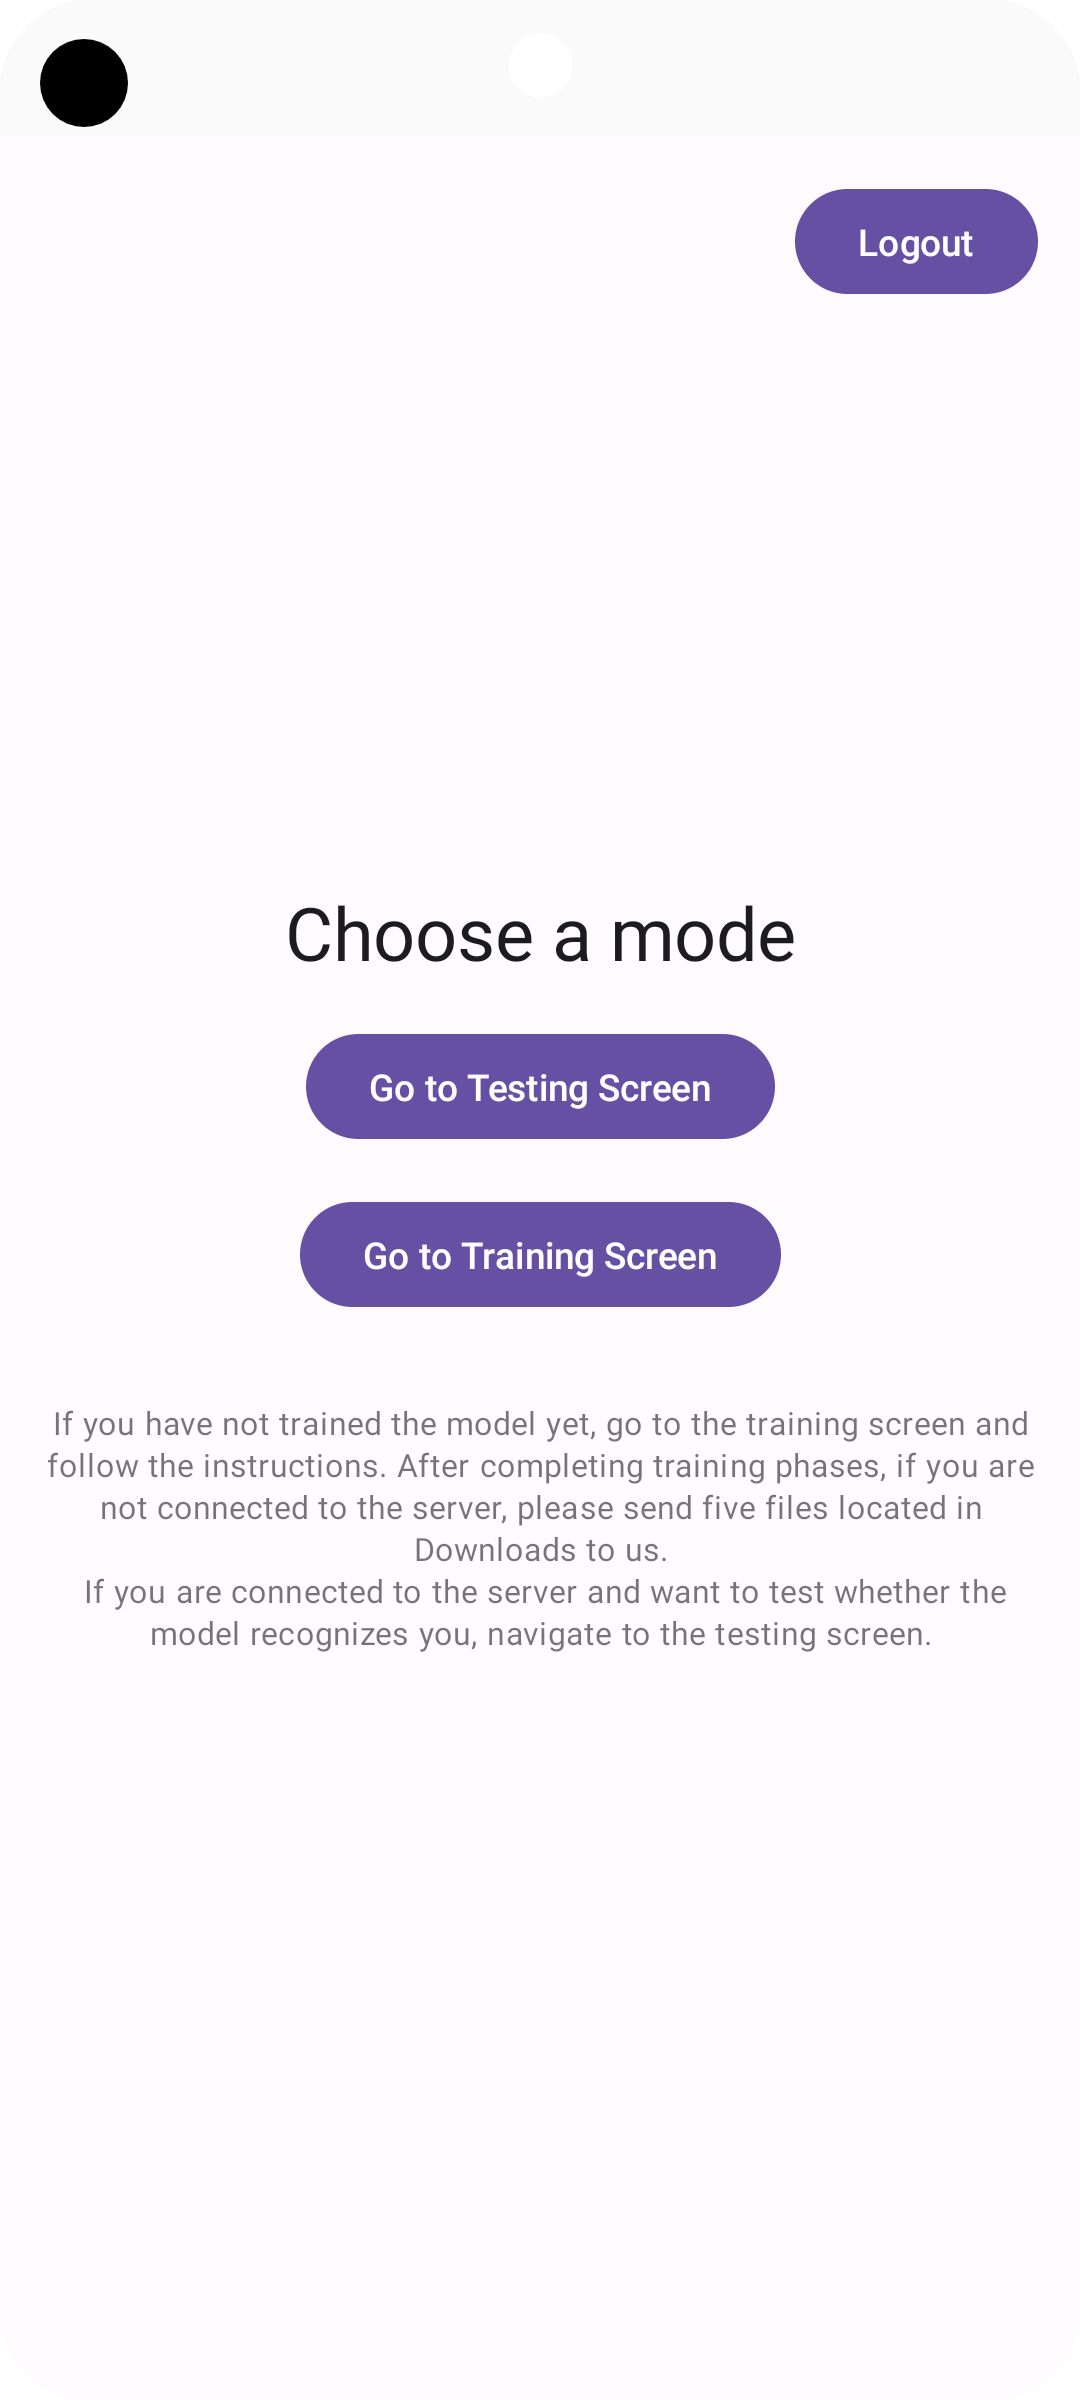
\includegraphics[width=0.32\linewidth]{images/home_screen.png}
	\caption{Home screen}
	\label{fig:home_screen}
\end{figure}

\begin{figure}[H]
	\centering
	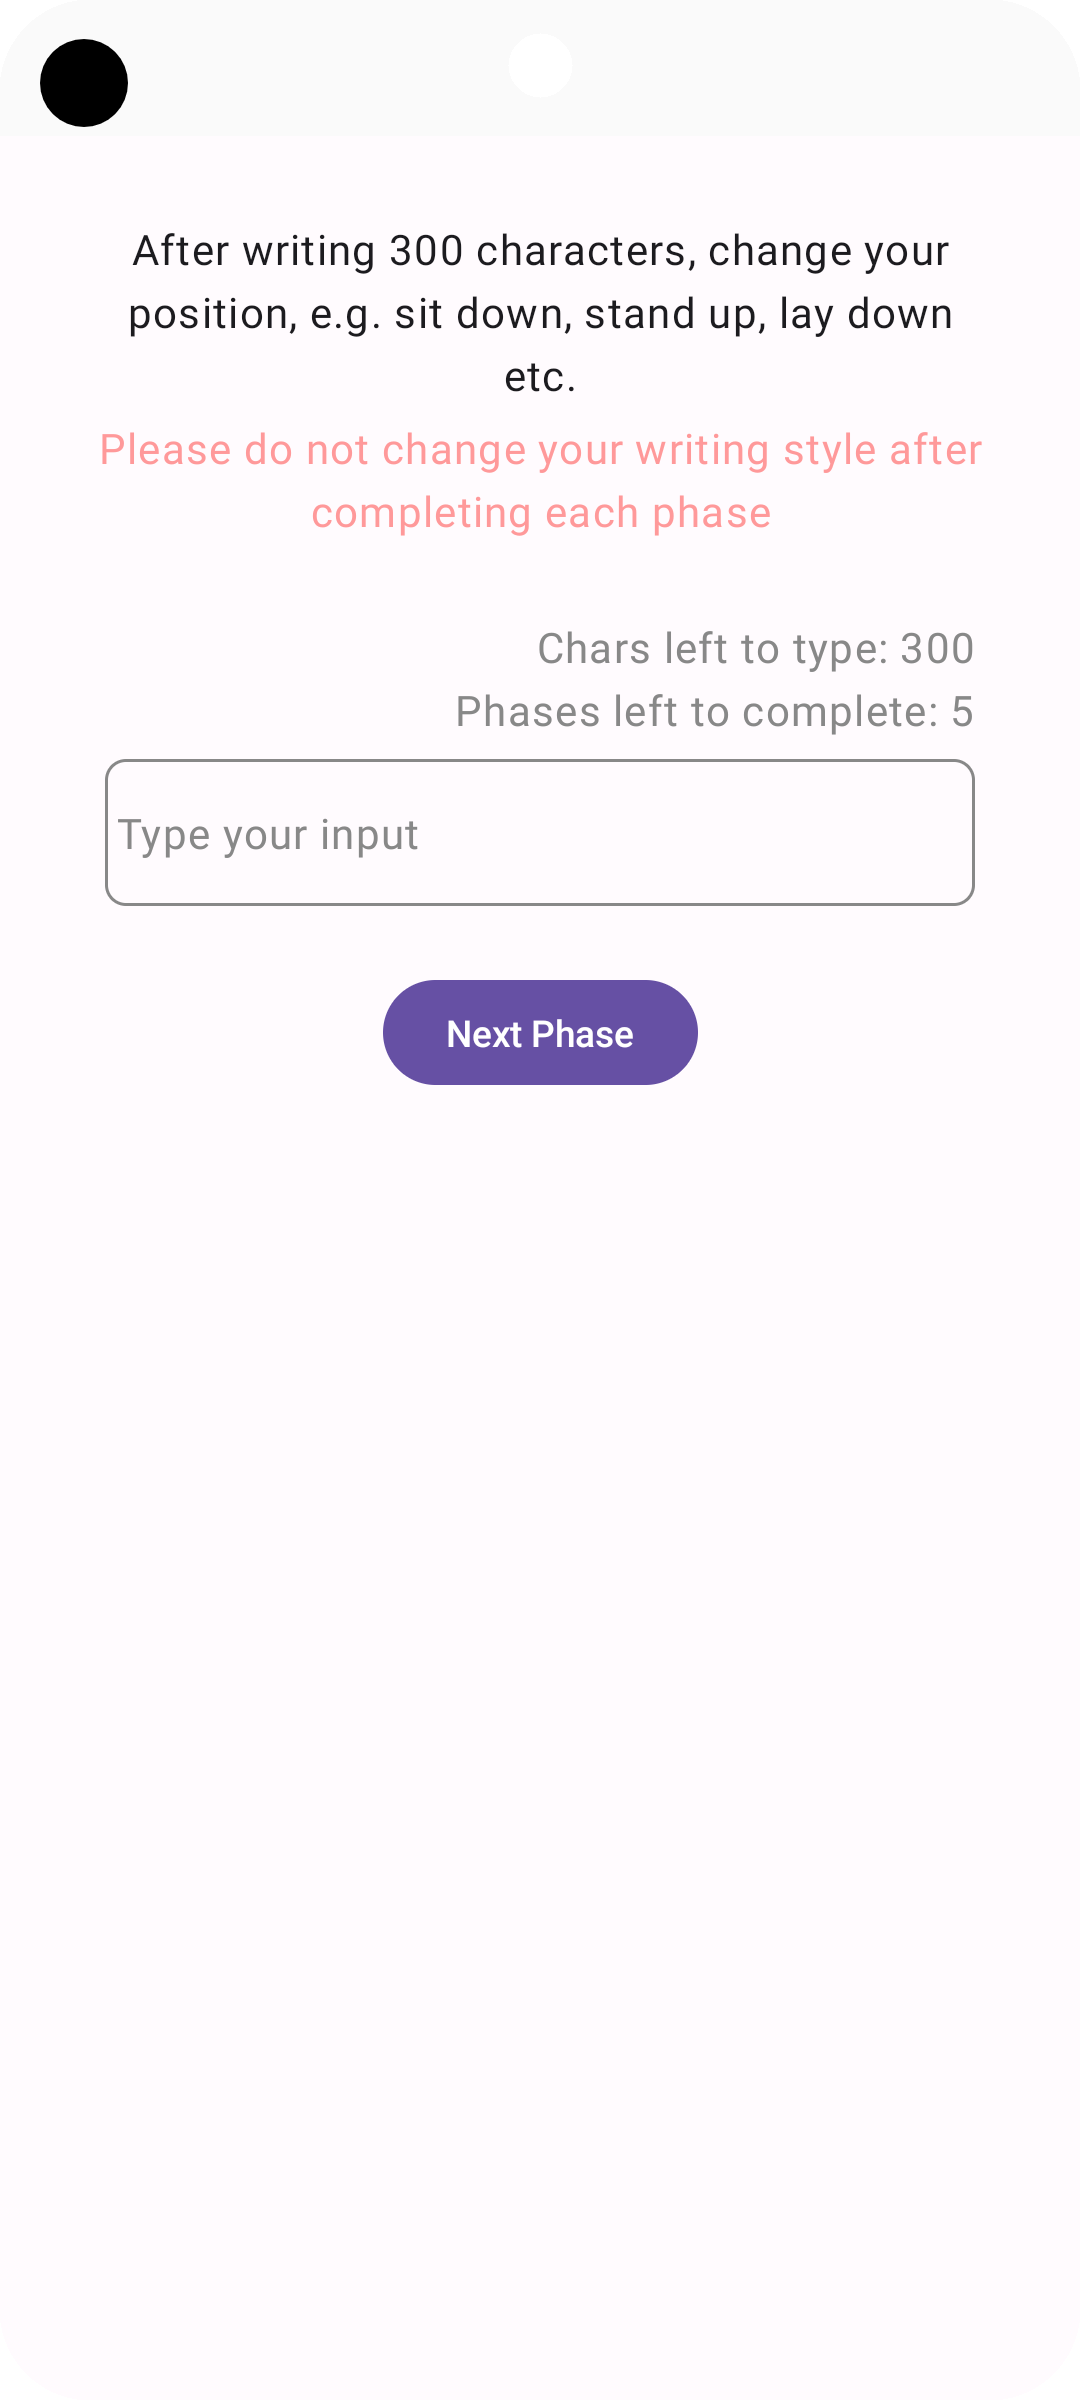
\includegraphics[width=0.32\linewidth]{images/training_screen.png}
	\caption{Training screen}
	\label{fig:training_screen}
\end{figure}

\begin{figure}[H]
	\centering
	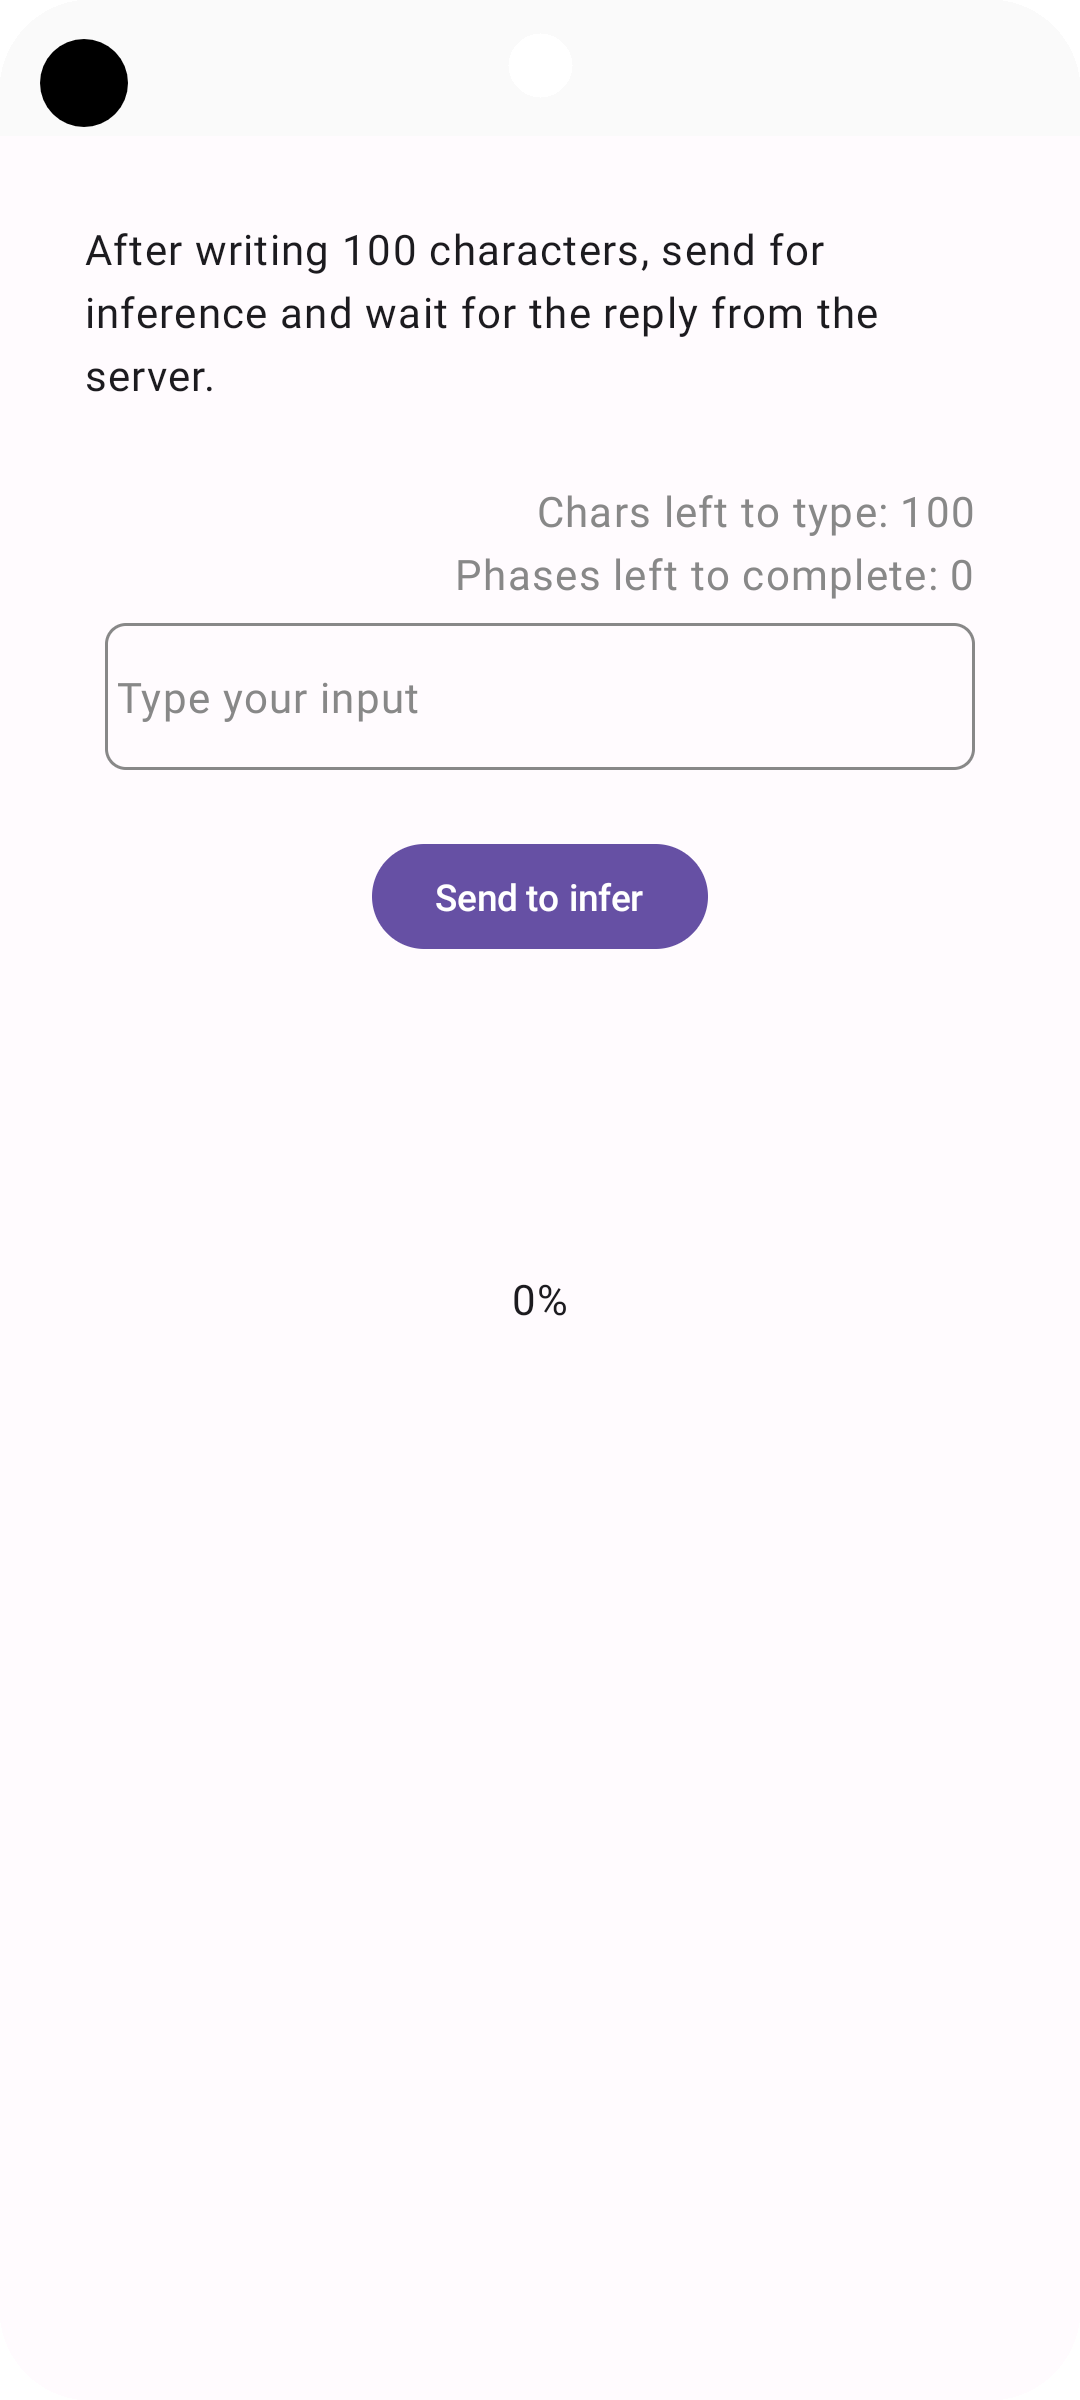
\includegraphics[width=0.32\linewidth]{images/testing_screen.png}
	\caption{Testing screen}
	\label{fig:testing_screen}
\end{figure}

\subsection{ideas}
Model View Controller and DataStore...

Data was modeled as...

Data was saved...

Application design...

Training screen...

Testing screen...

Communications with the server...

Data sent to the server and downloaded locally...

Those should be subsections